


\section{Gradient descent}
\label{sec:gd}
\subsection{Simple gradient descent}

As always in the context of ML, we want to minimize the cost function $E(\mathbf{θ})=\mC(\mx,g(\mathbf{θ}))$.
\begin{mybox}{Gradient descent}
The simplest gradient descent (GD) algorithm is characterized by the following \emph{update rule} for the parameters $\mathbf{θ}$. Initialize the parameters to some value $\mathbf{θ}_0$ and iteratively update the parameters according to the equation
\be
\label{eq:gdsimple}
\mathbf{v}_t = \eta_t \nabla_{θ} E(\mathbf{θ}_t),\quad \mathbf{θ}_{t+1} = \mathbf{θ}_t-\mathbf{v}_t
\ee 
where we have introduced the \emph{learning rate} $\eta_t$ (one hyperparameter of the model), that controls how big a step we should take in the direction of the gradient at time step $t$.
\end{mybox}
For sufficiently small choice of $\eta_t$, this method will converge to a \emph{local minimum} of the cost function, however this is computationally expensive. In practice, one usually specifies a ’schedule’ that decreases $\eta_t$ at long times (common schedules include power law and exponential decay in time).\footnote{Note that  Newton's method is a first-order approximation of GD method, which is not practical as it is a computationally expensive algorithm. However, Newton's method automatically adjusts the step size so that one takes larger steps in flat directions with small curvature and smaller steps in steep directions with large curavture. This gives an intuition of how to modify GD methods to get better results.}
The simple GD has the following limitations
\begin{enumerate}
\item GD finds local minima of the cost function.\\
Because in ML we are often dealing with extremely rugged landscapes with many local minima, this can lead to poor performance.
\item Gradients are computationally expensive to calculate for large datasets.
\item GD is very sensitive to choices of the learning rates.\\
Ideally, we would ’adaptively’ choose the learning rates to match the landscape.
\item GD treats all directions in parameter space uniformly.
\item GD is sensitive to initial conditions.
\item GD can take exponential time to escape saddle points, even with random initialization..
\end{enumerate}
These limitiations lead to generalized GD methods which form the backbone of much of modern DL and NN.
\subsection{Modified gradient descent}
\subsubsection{Stochastic gradient descent (SGD) with mini-batches}
\label{subsubsec:gdSGD}
\begin{mybox}{SGD}
		In SGD, we replace the actual gradient over the full data at each gradient descent step by an approximation to the gradient computed using a minibatch. This introduces stochasticity and decreases the chance that our fitting algorithm gets stuck in isolated local minima, as you cycle over all minibatches one at a time.\\
The update rule is
	\be
	\label{eq:gdstochastic}
	\mathbf{v}_t=\eta_t \nabla_{θ} E^{MB}(\mathbf{θ}),\quad \mathbf{θ}_{t+1} = \mathbf{θ}_t-\mathbf{v}_t.
	\ee 
\end{mybox}
\subsubsection{Algorithm gradient descent with momentum}
\marginpar{It has been argues that first-order methods (with appropriate initial conditions) can perform comparable to more expensive second-order methods, especially in the context of comples DL models.}
\begin{mybox}{GDM}
Introduce a ’momentum’ term into SGD which serves as a memory of the direction we are moving in parameter space. This helps the GD algorithm to gain speed in directions with persistent but small gradients even in the presence of stochasticity, while suppressing oscillations in high-curvature directions. The update rules is
\be 
\label{eq:gdmomentum}
\mathbf{v}_t = \gamma \mathbf{v}_{t-1}+\eta_t \nabla_{θ} E^{MB}(\mathbf{θ}_t), \quad \mathbf{θ}_{t+1} = \mathbf{θ}_t-\mathbf{v}_t,
\ee
where we have introduced a momentum parameter $\gamma \in [0,1]$. 
\end{mybox}
\begin{mybox}{NAG}
	A final widely used variant of gradient descent with momentum is called the Nesterov accelerated gradient (NAG). In NAG, rather than calculating the gradient at the current position, one calculates the gradient at the position momentum will carry us to at time  $t+1$ , namely, $ θ_t−γ v_{t−1}$ . Thus, the update becomes
	\be 
	\label{eq:gdNAG}
	\mathbf{v}_t = \gamma \mathbf{v}_t + \eta_t \nabla_{θ} E(\mathbf{θ}_t-\gamma \mathbf{v}_{t-1}),\quad \mathbf{θ}_{t+1} = \mt_{t}-\mathbf{v}_t.
	\ee 
\end{mybox}
\subsubsection{Methods that use the second moment of the gradient}
We would like to adaptively change the step size to match the landscape. This can be accomplished by tracking not only the gradient, but also the second moment of the gradient\footnote{Similar but avoiding the Hessian, which encodes local curvatures via second derivatives, as in Newton's method.}
\begin{mybox}{Root-mean-square propagation - RMSprop}
	In addition to keeping a running average of the first moment of the gradient, we also keep track of the second moment denoted by $\mathbf{s}_t=\mathbb{E}[\mathbf{g}^2_t]$. The update rule is 
	\be
	\label{eq:gdRMSprop}
	\mathbf{g}_t=\nabla_{θ} E(\mathbf{θ}),\; \mathbf{s}_t=\beta \mathbf{s}_{t-1} + (1-\beta) \mathbf{g}^2_t,\; \mathbf{θ}_{t+1}=\mathbf{θ}_t - \eta_t \frac{\mathbf{g}_t}{\sqrt{\mathbf{s}_t+\epsilon}},
		\ee 
		where $\beta$ controls the averaging time of the second moment and is typically taken to be about $\beta=0.9$, $\eta_t$ is typically chosen to be $10^{-3}$, and $\epsilon\propto 10^{-8}$ is a small regularization constant to prevent divergencies. It is clear from this formula that the learning rate is reduced in directions where the gradient is consistently large.
\end{mybox}
\begin{mybox}{ADAM}
	In ADAM, we keep a running average of both the first and second moment of the gradient and use this information to adaptively change the learning rate for different parameters. In addition to keeping a running average of the second moments of the gradient (i.e $\mathbf{m}_t= \mathbb{E}[\mathbf{g}_t], \mathbf{s}_t=\mathbb{E}[\mathbf{g}^2_t]$), ADAM performs an additional bias correction to account for the fact that we are estimating the first two moments of the gradient using a running average (denoted by the hat in the update rule). The update rule is given by (where multiplication and division are once again understood to be element-wise operations)
	\begin{align}
		\label{eq:gdADAM}
		\mathbf{g}_t &= \nabla_{θ} E(\mathbf{θ}), \quad \mathbf{m}_t =\beta_1 \mathbf{m}_{t-1} + (1-\beta_1) \mathbf{g}_t, \\
		\mathbf{s}_t &=\beta_2 \mathbf{s}_{t-1} + (1-\beta_2) \mathbf{g}^2_t,\quad \hat{\mathbf{m}}_t = \frac{\mathbf{m}}{1-(\beta_1)^t},\nonumber \\
		\hat{\mathbf{s}}_t &= \frac{\mathbf{s}_t}{1-(\beta_2)^t},\quad \mathbf{θ_{t+1}} = \mathbf{θ}_t - \eta_t \frac{\hat{\mathbf{m}}}{\sqrt{\hat{\mathbf{s}}_t} +\epsilon}\nonumber,
	\end{align}
where $\beta_1$ and $\beta_2$ set the memory lifetimes of the first and second moment (typically $\beta_{1,2} =\{0.9,0.99\}$ respectively, $\epsilon,\eta_t$ are same as in RMSprop).
\end{mybox}
The learning rates for RMSprop and ADAM can be set significantly higher than other methods due to their adaptive step sizes. For this reason, ADAM and RMSprop tend to be much quicker at navigating the landscape than simple momentum based methods.\footnote{Note that in some cases trajectories might not end up at the global minimum. This kind of landscape structure is generic in high-dimensional spaces where saddle points proliferate.}
\subsection{Practical tips for using GD}
Employ these tips for getting the best performance from GD based algorithms, especially in the context of deep neural networks (DNN)
\begin{enumerate}
	\item Randomize the data when making mini-batches.\\
	Otherwise, the GD method can fit spurious correlations resulting from the order in which data is presented.
	\item Transform your inputs.\\
	One simple trick for minimizing problems in difficult landscapes is to standardize the data by subtracting the mean and normalizing the variance of input variables. Whenever possible, also decorrelate the inputs. 
	\item Monitor the out-of-sample performance.\\
	Always monitor the performance of your model on a validation set (a small portion of the training data that is held out of the training process to serve as a proxy for the test set). If the validation error starts increasing then the model is beginning to overfit. Terminate the learning process. This \emph{early stopping} significantly improves performance in many settings.
	\item Adaptive optimization methods do not always have good generalization.\\
	Recent studies have shown that adaptive methods such as ADAM, RMSprop , and AdaGrad tend to have poor generalization to SGD or SGD with momentum, particularly in the high-dimensional limit (i.e. the number of parameters exceeds the number of data points). Although it is not clear at this state why sophisticated methods (e.g. ADAM, RMSprop, AdaGrad)  perform so well in training DNN such as generative adversarial networks (GANs), simpler procedures like properly-tuned plain SGD may work equally well or better in some applications.
\end{enumerate}







\section{Linear regression}
\label{sec:linearRegression}

\subsection{Least-square regressions -frequentist}
We'll consider ordinary least squares regression problem in which the "error function" is defined as the square from the deviation of our linear predictor to the true response. 
\begin{mybox}{OLS}
\emph{Ordinary least squares linear regression} (OLS) is defined as the minimization of the $L_2$ norm of the difference between the response $y_i$ and the predictor $g(\mx^{(i)};\textbf{w})=\textbf{w}^T \mx^{(i)}$:
\be 
\label{eq:lregOLS}
\min_{\textbf{w} \in \mR^p} \norm{\mX \textbf{w} -\my}^2_2 = \min_{\textbf{w} \in \mR^p}\sum_{i=1}^n (\mw^T \mx^{(i)} - y_i)^2.
\ee
Where \ref{eq:lregOLS} is the minimization of the loss function of OLS.\\
We are looking to find the parameters $\mw$ which minimize the $_2$ error. Geometrically speaking, the predictor function $g$ defines a hyperplane in $\mR^p$. Minimizing the least squares error is therefore equivalent to minimizing the sum of all projections (i.e. residuals) for all points$\mx^{(i)}$ to this hyperplane. If $\rank (\mX)=p$ , namely, the feature predictors  $\mX_{:,1},\dots,\mX_{:,p}$  are linearly independent, then there exists unique solution to this problem, which we denote as $\hat{\mw}_{LS}$:
\be 
\label{eq:lregOLSsolution}
\hat{\mw}_{LS} = \arg \min_{\mw \in \mR^p} \norm{\mX \mw - \my}^2_2 = (\mX^T \mX )^{-1} \mX^T \my,
\ee 
where we have assumed that $\mX^T\mX$ is inertible, which is often the case when $n\gg p$ (i.e. method works if number of data points exceeds number of features). The best fit of our data $\mX$ is
\be 
\label{eq:lregOLbestfit}
\hat{\my} = \mX \hat{\mw}_{LS} = \underbrace{\mX (\mX^T \mX)^{-1} \mX^T}_{\equiv P_{\mX}},
\ee 
where $P_{\mX}$ is the projection matrix which acts on $\my$ and projects it onto the column space of $\mX$, which is spanned by the predictors $\mX_{:,1},\dots,\mX_{:,p}$.
\end{mybox}
Note how we found the optimal solution $\hat{\mw}_{LS}$ in one shot, without doing any sort of iterative optimization.\\
What are the errors of OLS such that we can evaluate its performance according to \ref{subsec:performanceeval} ?\footnote{As we have seen, the difference between learning and fitting lies in the prediction on ’unseen’ data.}\\
We find that the average \emph{generalization error} for this method to be
\be 
\abs{\bar{E}_{in}-\bar{E}_{out}} = \sigma^2 \abs{(1-\frac{p}{n}) -(1+\frac{p}{n})}= 2 \sigma^2 \frac{p}{n}.
\ee 
\begin{mybox}{}
	This implies: If we have $p\gg n$ (i.e. high-dimensional data), the generalization error is extremely large, meaning the model is not learning. Even when we have $p\approx n$, we might still not learn well due to the intrinsic noise $\sigma^2$.
\end{mybox}
One way to ameliorate this is to use regularization. We will mainly focus on two forms of regularization which are introduced in the following:\\
the first one employs an $L_2$ penalty and is called \emph{Ridge regression}, while the second uses an $L_1$ penalty and is called $LASSO$.
\subsection{Regularized Least-square regressions-frequentist}
Due to poor generalization, regularization is necessary, in particular  in the \emph{high-dimensional limit} ($p\gg n$). Regularization typically leads to better generalization. 
\begin{mybox}{Idea behind regularization}
	Due to the equivalence between the constrained and penalized form of regularized regression, we can regard the regularized regression problem as an un-regularized problem but on a \emph{constrained set of parameters}. Since the size of the allowed parameter space (e.g. $\mw \in \mR^p$ when un-regularized vs. $\mw \in C \subset \mR^p$ when regularized) is roughly a proxy for model complexity, solving the regularized problem is in effect \textbf{solving the un-regularized problem with a smaller model complexity class}. This implies that we are \textbf{less likely to overfit}.
\end{mybox}
Why is that so ?\\
Let's say you are a young Physics student taking a laboratory class where the goal of the experiment is to measure the behaviour of several different pendula and use that to predict the formula (i.e. model) that determines the period of oscillation. In you investigation you would probably recod many things in an effort to give yourself the best possible chance of determining the unknown relationship, perhaps writing down the temperature of the room, any air currents, if the table were vibrating, etc. What you have done is create a high-dimensional dataset for yourself. However you actually possess an even higher-dimensional dataset than you probably would admit to yourself, e.g. whether it is Alice's birthday or whether you found a penny this morning, but you almost assuredly haven't written these down in your notebook. Why not ? The reason is because \emph{you entered the classroom with strongly held \textbf{prior beliefs} that none of those things affect the physics which takes place in that room}. What is serving you here is the \emph{intuition} that probably only a few things matter in the physics of pendula. Hence again you are approaching the experiment with prior beliefs about how many features you will need to pay attention to in order to predict what will happen when you swing an unknown pendulum.\\
The point is that we live in a high-dimensional world of information and while we have good intuition about what to write down in our notebook for well-known problems, often in the field of ML we cannot say with any confidence a priori \emph{what} the small list of things to write down will be, but we can at least \textbf{use regularization to help us enforce that the list not be too long} so that we don't end up predicting that the period of a pendulum depends on Bob having a cold on Wednesdays.
\subsubsection{Ridge-Regression}
\begin{mybox}{Ridge-Regression}
	We now add to the least squares loss function a \emph{regularizer} defined as as the $L_2$ norm of the parameter vector we wish to optimize over. In Ridge-Regression, the regularization penalty is taken to be the $L_2$-norm of the parameters 
	\be 
	E_{Ridge} = \lambda \norm{\mw}^2_2 = \lambda \mw^T\mw = \lambda \sum_{\gamma=1}^p w_\gamma w_\gamma.
	\ee 
	Thus, the model is fit by minimizing the sum of the in-sample error and the regularization term
	\be 
	\label{eq:lregRidge}
	\hat{\mw}_{Ridge} (\lambda) = \arg \min_{\mw \in \mR^p}\left(\norm{\mX \mw - \my}^2_2 + \lambda \norm{\mw}^2_2\right)
	\ee 
	Notice that the parameter $\lambda$ controls how much we weigh the fit and regularization term.
	The solution/estimate is found by differentiating w.r.t $\mw$
	\be 
	\label{eq:lregRidgeSol}
	\hat{\mw}_{Ridge}(\lambda)=\frac{\hat{\mw}_{LS}}{1+\lambda} 
	\ee 
	where the  equality via \ref{eq:lregOLSsolution} holds for orthogonal $\mX$. This implies that the ridge estimate is merely the least squares estimate scaled by a factor $(1+\lambda)^{-1}$.
	This problem is equivalent to the following \emph{constrained} optimization problem
	\be 
	\hat{\mw}_{Ridge}(t) ) \arg \min_{\mw \in \mR^p: \norm{\mw}^2_2 \leq t} \norm{\mX \mw -\my}^2_.2.
	\ee 
	Thus, by adding a regularization term, $\lambda \norm{\mw}^2_2$, to our least squares loss function, we are effectively constraining the magnitude of the parameter vector learned from the data. The solution
\end{mybox}
One can furthermore derive a relation (via singular value decomposition (SVD) on X) between the fitted vector $\hat{\my}=\mX\hat{\mw}_{Ridge}$ and the prediction made by least squares linear regression
\be 
\hat{y}_{Ridge} =\mX \hat{\mw}_{Ridge} \leq \mX \hat{\my} \equiv \hat{\my}_{LS}.
\ee 
It is clear that in order to compute the fitted vector $\hat{\my}$, both Ridge and least squares linear regression have to project $\my$ to the column space of $\mX$. The only difference is that Ridge regression further shrinks each basis component $j$ by a factor $d^2_j/(d^2_j+\lambda)$, where $d_1\geq d_2\geq \dots d_p \geq 0$ are the singular values of $\mX$.
\begin{mybox}{}
	It is considered good practice to always check the performance for the given model and data as a function of $\lambda$.
\end{mybox}
If increasing $\lambda$  simply degrades performance, we are most likely not undersampled.
\subsubsection{LASSO and Sparse Regression}
\begin{mybox}{LASSO}
	Now we add an $L_1$ regularization penalty, conventionally called ’least absolute shrinkage and selection operator’ (LASSO). The penalty is the $L_1$-norm of the parameters (sum of absolute values of parameters)
	\be 
	E_{LASSO}= \lambda \norm{\mw}_1 = \lambda \sum_{\gamma=1}^p \abs{\mw_\gamma}
	\ee 
	LASSO in the penalized form is defined by the following regularized regression problem
	\be 
	\label{eq:lregLASSO}
	\hat{\mw}_{LASSO}(\lambda) = \arg \min_{\mw \in \mR^p} \norm{\mX \mw - \my }^2_2 + \lambda \norm{\mw}_1.
	\ee 
	Obtaining a solution is not that easy, assuming $\mX$ to be orthogonal one finds a so-called threshold function (compare \ref{fig:lassovsridge})
	\be 
	\label{eq:lregLASSOSol}
	\hat{w}^{LASSO}_j(\lambda)= \text{sign}(\hat{w}^{LS}_j)\left[\abs{\hat{w}^{LS}_j}-\lambda\right]_+
	\ee 
	where $(x)_+$ denotes the positive part of $x$ and $\hat{w}^{LS}_j$ is the $j$th component of \ref{eq:lregOLSsolution}.\\
	In general, LASSO tends, in contrast to Ridge, to given sparse solutions, meaning many components of $\hat{\mw}_{LASSO}$ are zero. Looking at the behaviour of weights of LASSO and Ridge depending on the regularization parameter, one observes that LASSO, unlike Ridge, sets feature weights to zero leading to sparsity.
\end{mybox}
\begin{figure}[h!]
	\centering
	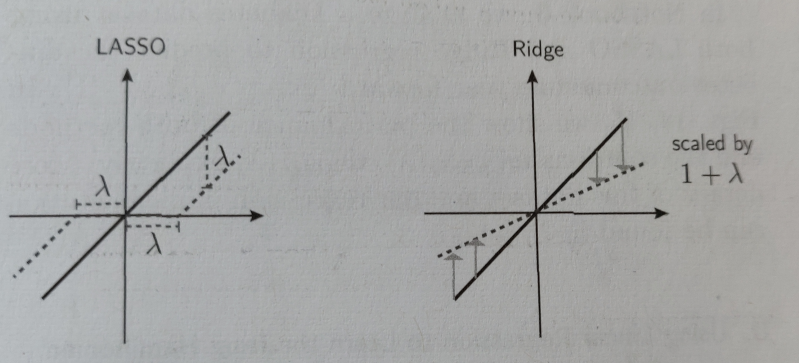
\includegraphics[width=0.7\linewidth]{gfx/LassoVsRidge}
	\caption{}
	\label{fig:lassovsridge}
\end{figure}
\begin{mybox}{On the hyperparameter}
	The regularization parameter $\lambda$ affects the weights (features) the model (LASSO, Ridge) learns on a data set.
\end{mybox}

\subsubsection{A note on LASSO and Ridge}
Note that both LASSO and Ridge regression are convex in  $\mw$ . What's more, Ridge is actually a strictly convex problem (assuming  $\lambda >0$ ) due to presence of $L_2$ penality. In fact, this is always true regardless of  $\mX$  and so the ridge regression solution is always well-defined.

In contrast, LASSO is not always strictly convex and hence by convexity theory, it need not have a unique solution. The LASSO solution is unique under general conditions, for example, when  $\mX$  has columns in general position. To mitigate this, one can define a modified problem called the elastic net such that the function we want to minimize is always strictly convex:
\bse 
\min_{\mw \in \mR^p}\norm{\mX \mw -\my}^2_2 + \lambda \norm{\mw}_1+\delta \norm{\mw}^2_2
\ese 
where  $λ,δ\geq 0$  are regularization parameters. Now aside from uniqueness of the solution, the elastic net combines some of the desirable properties (e.g. prediction) of ridge regression with the sparsity properties of the LASSO.
\subsubsection{Another note being a general comment on regularization}
Comparing the performance of OLS, LASSO and Ridge for the $1D$ Ising model via the coefficient of determination \ref{eq:errorR2} by looking at the parameter space of the hyperparameter $\lambda$, one can draw the following conclusions.\\
Choosing whether to use Ridge or LASSO regression turns out to be similar to fixing gauge degrees of freedom.
\begin{mybox}{Picking a regularization scheme}
	Different regularization schemes can lead to learning equivalent models but in different ’gauges’. Any information we have about the symmetry of the unknown model that generated the data should be reflected in the definition of the model and the choice of regularization.
\end{mybox}

\subsubsection{A general perspective on regularizers}
\begin{mybox}{On the hyperparameter}
	The \textbf{hyperparameter} $\lambda$ involved in e.g. LASSO and Ridge is usually predetermined, which means that it is not part of the regression process. Our learning performance and solution depends strongly on $\lambda$, thus it is vital to choose it properly. As discussed in \ref{subsec:priors}, one approach is to assume an \emph{uninformative prior} on the hyper-parameters, $p(\lambda)$, and average the posterior over all choices of $\lambda$ following this distribution. However, this comes with a large computational cost. Therefore, is is simpler to choose the regularization parameter through some optimization procedure.
\end{mybox}






\subsection{Bayesian formulation of linear regression}
\label{subsec:lregBayesian}
In the formal statistical treatment of regression, the goal is to estimate the \emph{conditional expectation} of the depndent variable given the value of the independent variable (sometimes called the covariate). To connect linear regression to the Bayesian framework, we use \ref{eq:bayesianFreqConnectionModel}. In combination with \ref{eq:bayesLogLikelihood}, we get
\bse 
l(\mt)=-\frac{1}{2\sigma^2} \sum_{i=1}^n(y_i-\mw^T \mx^{(i)})^2-\frac{n}{2} \log(2 \pi  \sigma^2) = -\frac{1}{2\sigma^2} \norm{\mX \mw -\my}^2_2 + const.
\ese
\begin{mybox}{} 
By comparing this with \ref{eq:lregOLSsolution}, it is clear that 
 performing least squares is the same as maximizing the log-likelihood of this model.
\end{mybox}

 \subsubsection{Regularization }
 What about adding regularization?
 \begin{mybox}{}
 The MAP estimate  \ref{eq:bayesMAPestimate} corresponds to regularized linear regression, where the choice of prior determines the type of regularization.
 \end{mybox}
The equivalence between MAP estimation with a Gaussian prior and Ridge regression is established by comparing \ref{eq:bayesMAPestimatorGaussianPrior} and Ridge regression \ref{eq:lregRidgeSol} with $\lambda \equiv \sigma^2/\tau^2$. An analogous derivation holds for LASSO \todo{todo ?}.

\subsection{Outlook from linear regression}
Linear regression can be applied to model non-linear relationships between input and response. This can be done by replacing the input $\mx$ with some non-linear function $\phi(\mx)$. Note that doing so preserves the linearity as a function of the parameters $\mw$, since the model is defined by their inner product $\phi^T(\mx) \mw$. This method is known as \emph{basis function expansion}.\footnote{Look into ML for physicists review for references.}







\section{Logistic Regression}
\label{sec:logisticRegression}
So far we have focused on learning from datasets for which there is a ’continuous’ output. However, a wide variety of problems, such as \emph{classification}, are concerned with outcomes taking the form of discrete variables (i.e. \emph{categories}).
\begin{example}
	For example, we may want to detect if there is a cat or a dog in an image.
\end{example}
We will now introduce \emph{logistic regression} which deals with binary, dichotomous outcomes (.e.g. True or False, Success or Failure,etc.).
\subsection{Mathematical set-up}
\subsubsection{Binary classification}
\label{subsubsec:classBinary}
Throughout this section, we consider the case where the dependent variables $y_i\in \Z$ are discrete and only take values from $m=0,\dots,M-1$ (which enumerate the $M$ classes). The goal is to predict output classes from the design matrix $\mX\in \mR^{n\times  p}$ made of $n$ samples, each of which bears $p$ features. The primary goal is to identify the classes to which new unseen samples belong.
\subsubsection{Multi-class classification}
\label{subsubsec:classMultiClass}
For multi-class classification, we can not only look at binary classification (in which the labels are dichotomous variables). One approach is to treat the label as a vector $\my_i\in \Z^M_2$, namely a binary string of length $M$ with only one component of $y_i$ being $1$ and the rest zero.
\begin{example}
	For example, $\my_i=(1,0,\dots,0)$ means data the sample $\mx_i$ belongs to class $1$.
\end{example}




\subsection{Classifiers}
Given $\mx_i$, the classifier returns the probability of being in category $m$. The following perceptron is an example of \emph{hard} classification, each datapoint is assigned to a category (i.e. $y_i=0$ or $y_i=1$). A \emph{soft} classifier on the other hand gives the probability of a given category as an output.\\
The classifiers do this by using threshold functions, which are discussed in the following \ref{subsubsec:thresholdfct}.\\
In many cases, it is favourable to work with a soft classifier.
\subsubsection{On threshold function functions}
\label{subsubsec:thresholdfct}
	A threshold function is a function that maps its input $\mx$ (a real-valued vector) to an output value $f(x)$ (a single binary value).
One simple way to get a discrete output is to have sign (or threshold) functions that map the output of a linear regressor to $\{0,1\}$. The following are possible:
\begin{enumerate}
	\item Step functions (perceptrons) given by the \emph{sign} function 
\be
\label{eq:logRegsign}
\sigma(s_i)=\text{sign}(s_i)= \left\{\begin{array}{ll}
	1 & \text{if } s_i\geq 0 \\
	0 & \text{otherwise} \\
\end{array}  \right\}
\ee
are employed for hard classification.
\item The \emph{logistic} (or \emph{sigmoid}) function (i.e. Fermi functions)
\be 
\label{eq:logRegSigmoid}
\sigma(s) = \frac{1}{1+e^{-s}}, \quad 1-\sigma(s) = \sigma(-s).
\ee 
\item The hyperbolic tangent 
\todo{Put definition here}
\be 
\label{eq:logRegHyperbolicTangent}
\tanh(z) 
\ee 
\item Rectified linear units (ReLUs) 
\item Leaky rectified linear unity (leaky ReLUs)
\item Exponential linear units (ELUs)
\end{enumerate} 














\subsection{Perceptron Learning Algorithm (PLA)}
Before delving into the details of logistic regression, it is helpful to consider a slightly simpler classifier.
\begin{mybox}{Perceptron crude idea}
	Consider a linear classifier that categorizes examples using a weighted linear-combination of the features and an additive offset:
	\be 
	\label{eq:logRegPerceptron}
	s_i = \mx^T_i \mw + b_0  \equiv \mathbf{\textbf{x}}^T_i \mathbf{\textbf{w}},
	\ee 
	where we use the short-hand notation $\mathbf{\textbf{x}}_i=(1,\mx_i)$ and $\mathbf{\textbf{w}}=(b_0,\mw)$. This function takes values on the entire real axis. IN the case of logistic regression, however, the labels $y_i$ are discrete variables. Using the sign function \ref{eq:logRegsign} to create discrete outputs via hard classification, we obtain the \emph{perceptron} model.\\
	In the modern sense, the perceptron is an algorithm for learning a binary classifier called a  \emph{threshold function}, see \ref{subsubsec:thresholdfct}.
\end{mybox}
\subsubsection{The algorithm}


Suppose that we're given a set of $N$ observations each bearing $p$ features, $\mx_n=(x_1^{(n)},\cdots, x_p^{(n)})\in\mathbb{R}^p$, $n=1,\cdots, N$. The goal of binary classification is to relate these observations to their corresponding binary label $y_n \in\{+1,-1\}$. Concretely, this amounts to finding a function $h: \mathbb{R}^p\rightarrow \{+1,-1\}$ such that $h(\mx_n)$ is ideally the same as $y_n$. 
\begin{mybox}{Perceptron} 
	A \emph{perceptron} accomplishes this feat by utilizing a set of weights $\textbf{w}=(w_0,w_1,\cdots, w_d)\in\mathbb{R}^{p+1}$ to construct $h$ so that labelling is done through
\be 
	h(\textbf{x}_n)=\text{sign }\left(w_0+\sum_{i=1}^p w_ix_i^{(n)}\right) =\text{sign }(\textbf{w}^T\textbf{x}_n),
	\ee 
	
	where $\textbf{x}_n=(1,x_1^{(n)},\cdots, x_p^{(n)}) = (1,\mx_n)$. The perceptron can be viewed as the zero-temperature limit of the logistic regression where the sigmoid (Fermi-function) becomes a step function.
	
\end{mybox}

PLA begins with randomized weights. It then selects a point from the training set at random. If this point, say, $\textbf{x}_n$, is misclassified, namely, $y_n\neq \text{sign }(\textbf{w}^T\textbf{x}_n)$, weights are updated according to 
\be 
\textbf{w}\leftarrow \textbf{w}+ y_n\textbf{x}_n
\ee 
Otherwise, $\textbf{w}$ is preserved and PLA moves on to select another point. This procedure continues until a specified threshold is met, after which PLA outputs $h$. It is clear that PLA is an online algorithm since it does not treat all available data at the same time. Instead, it learns the weights as it progress along data points in the training set one-by-one. The update rule is built on the intuition that whenever a mistake is encountered, it corrects its weights by moving towards the right direction. 












\subsection{Definition of logistic regression - Bayesian}
This is a binary classification problem, see \ref{subsubsec:classBinary}.
Here we define logistic regression and discuss the minimization of its corresponding cost function (the \emph{cross entropy}). 
\begin{mybox}{Logistic regression}
	Logistic regression is the canonical example of a soft classifier. In logistic regression, the probability that a data point $\mx_i$ belongs to a category $y_i = \{0,1\}$ is given by 
	\begin{align*}
		P(y_i=1|\mx_i,\mt)&= \frac{1}{1+e^{-\mathbf{\textbf{x}}^T_i \mt}} = \sigma(\mathbf{\textbf{x}}^T_i \mathbf{\textbf{w}})\\
		P(y_i=0|\mx_i,\mt) &= 1-P(y_i=1|\mx_i,\mt)
	\end{align*}
	where $\mt = \mathbf{\textbf{w}}$ are the weights we wish to learn from the data. The cost function of logistic regression, the \emph{cross entropy}, is found to be
	\be 
	\label{eq:logregCrossEntropy}
	\mC(\mathbf{\textbf{w}} )= \sum_{i=1}^n \left[-y_i \log \sigma(\mathbf{\textbf{x}}^T_i \mathbf{\textbf{w}}) -(1-y_i) \log\left(1-\sigma(\mathbf{\textbf{x}}^T_i \mathbf{\textbf{w}})\right)\right].
	\ee 
	In practice, we usually implement the cross-entropy (like in linear regression) with additional regularization terms, usually $L_1$ and $L_2$ regularization.
\end{mybox}
\begin{mybox}{Minimizing the cross entropy}
	The cross entropy is a convex function of the weights $\textbf{w}$ and, therefore, any local minimizer is a global minimizer. Minimizing this cost function leads to 
	\be 
	\label{eq:logregCrossEntropyMinimized}
	0 = \mathbf{\nabla} \mC(\textbf{w}) = \sum_{i=1}^n \left[\sigma(\textbf{x}^T_i \textbf{w}) - y_i\right]\textbf{x}_i.
	\ee 
	In words, the gradient points in the sum of training example directions weighted by the difference between the true label and the probability of predicting that label.
	Equation \ref{eq:logregCrossEntropyMinimized} defines a transcendental equation for $\textbf{w}$, the solution of which, unlike linear regression, cannot be written in a closed form. For this reason, one must use numerical methods such as \ref{sec:gd} to solve this optimization problem.
\end{mybox}\footnote{However, as a word of caution, note there is a generic instability in the MLE procedure for linearly separable data)}
In the notebooks, one looks at two examples to train a logistic regressor to classify binary data.
We call \emph{one-hot} a group of bits where only one bit is $1$ and all others $0$, i.e. representing states: $\ket{1}=(1,0,\dots,0), \ket{2}=(0,1,0,\dots,0)$.
\subsubsection{On the 2d Ising example}
Given an Ising state, we would like to classify whether it belongs to the ordered or the disordered phase, without any additional information other than the spin configuration itself. This categorical ML problem is well suited for logistic regression, and will thus consist of recognizing whether a given state is ordered by looking at its bit configurations. Notice that, for the purposes of logistic regression, the $2D$ spin state of the Ising model will be flattened out to a $1D$ array, so it will not be possible to learn information about the structure of the contiguous ordered $2D$ domains. SUch information can be incorporated using deep convolutional neural networks.\\
We use both ordered and disordered states to train the logistic regressor and, once the supervised training procedure is complete, we will evaluate the performance of our classification model on unseen ordered, disordered, and near-critical states. Here, we deploy the \emph{liblinear} routine (the default for Scikit' s logistic regression) and stochastic gradient descent to optimize the logistic regression cost function with $L_2$ regularization. We define the accuracy of the classifier as the percentage of correctly classified data points. Comparing the accuracy on the training and test data, we can study the degree of overfitting.\\
Similar to the linear regression examples, we find that there exists a sweet spot for the SGD regularization strength $\lambda$ that results in optimal performance of the logistic regressor.
\subsubsection{SUSY }
Here we will use logistic regression in an attempt to find the relative probability that an event is from a signal or a background. Is a good classification problem with noisy data, how to discriminate against the background ? Some signal events look background-like, and some background events look signal-like to our discriminator.
\subsection{SoftMax regression}
\label{subsec:logregSoftMax}
In this section we generalize logistic regression to the case of multiple categories which is called \emph{SoftMax regression}. This is a multi-class classification problem \ref{subsubsec:classMultiClass}.\\
For general categorical data, $y$ can then take on $M$ values so that $y\in \{0,1,\dots, M-1 \}$. For each datapoint $i$, define a vector $y_{im} \equiv [\my_i]_{m}$, whichs refers to the $m^\prime$-th component of vector $\my_i$, called a \emph{one-hot} vector, such that
\be
y_{im} = \left\{ \begin{array}{ll}
	1, & \text{if } y_i = m \\
	0, & \text{otherwise}. \\
\end{array}	\right\}
\ee 
\begin{mybox}{SoftMax regression}
	The probability of $\mx_i$ being in class $m^\prime$ is given by
	\be
	\label{eq:logregSoftMaxfct} 
	\hat{y}_{im (\tw) = p(yi=m^\prime | \tx_i;\tw) \equiv }P(y_{im^\prime} =1 | \mx_i,\{\textbf{w}_k\}^{M-1}_{k=0})=\frac{e^{-\textbf{x}^T_i \textbf{w}_{m^\prime}}}{\sum_{m=0}^{M-1} e^{-\textbf{x}^T_i \textbf{w}_m}},
	\ee 
	where $y_{im^\prime} \equiv [\my_i]_{m^\prime}$ refers to the $m^\prime$-th component of vector $\my_i$. This is known as the \emph{SoftMax} function. The generalized cost function reads
	\begin{align}
	\label{eq:logregSoftMaxcostFct}
	\mC(\textbf{w}) &= - \sum_{i=1}^n \sum_{m=0}^{M-1} \left[ y_{im} \log P(y_{im}=1|\mx_i, \textbf{w}_m) \right.. \\
	&\left. + (1-y_{im }) \log\left(1-P(y_{im} =1 |\mx_i ,\textbf{w}_m)\right)\right],
	\end{align} 
	which reduces to the cross entropy \ref{eq:logregCrossEntropy} for $M=1$, i.e. for only two possible classes.
\end{mybox}




\section{Ensemble Methods - On combining models}
\label{sec:ensembles}
\subsection{Introduction}
Ensemble methods combine predictions from multiple, often weak, statistical models to improve predictive performance. Ensemble methods, such as random forests, and boosted gradient trees, such as XGBoost, undergird many of the winning entries in data science competitions such as Kaggle, especially on structured datasets. Note that Neural Networks generally perform better than ensemble methods on unstructured data, images and audio. Even in the context of NN, it is common to combine predictions from multiple neural networks to increase performance on tough image classification tasks.
\subsubsection{Motivation}
\label{subsubsec:ensemblesMotivation}
We will give an overview of ensemble methods and provide rules of thumb for when and why they work.\\
On one hand, the idea of training multiple models and then using a weighted sum of the predictions of all these models is very natural. On the other hand, one can also imagine that the ensemble predictions can be much worse than the predictions from each of the individual models that constitute the ensemble, especially when pooling reinforces weak but correlated deficiencies in each of the individual predictors. Thus, it is important to understand when we expect ensemble methods to work.\\
As we saw in \ref{subsubsec:biasvarianceMathematicalEnsemble}, the key to determining when ensemble methods work is the degree of correlation between the models in the ensemble.
\subsubsection{Benefits of Ensemble Methods before diving in}
Three distinct shortcomings that are fixed by ensemble methods are: statistical, computational, and representational.\\
The first reason is statistical. When the learning set is too small, a learning algorithm can typically find several models in the hypothesis space $\mH$ that all give the same performance on the training data. Provided their predictions are uncorrelated, averaging several models reduces the risk of choosing the wrong hypothesis. The second reason is computational. Many learning algorithms rely on some greedy assumption or local search that may get stuck in local optima. As such, an ensemble made of individual models built from many different starting points may provide a better approximation of the true unknown function than any of the single models. Finally, the third reason is representational. In most cases, for a learning set of finite size, the true function cannot be represented ba any of the candidate models in $\mH$. By combining several models in an ensemble, it may be possible to expand the space of representable functions and to better model the true function.\\
\\ 
The increase in representational power of ensembles comes from the fact that it is more advantageous to combine a group of simple hypotheses than to utilize a single arbitrary linear classifier. This of course comes with the price of introducing more parameters to our learning procedure. But if the problem itself can never be learned through a simple hypothesis, then there is no reason to avoid applying a more complex model. Since ensemble methods reduce the variance and are often easier to train than a single complex model, they are a powerful way of increasing representational power (also called expressivity in the ML literature).\\
\\
How should we construct ensembles ?\\
\begin{enumerate}
	\item Try to randomize ensemble construction as much as possible to reduce the correlations between predictors in the ensemble. This ensures that our variance will be reduced while minimizing an increase in bias due to correlated errors.
	\item The ensembles will work best for procedures where the error of the predictor is dominated by the variance and not the bias. Thus, these methods are especially well suited for unstable procedures whose results are sensitive o small changes in the training dataset.
	\item Although the discussion above was derived in the context of continuous predictors such as regression, the basic intuition behind ensembles applies equally well to classification tasks. Using an ensemble allows one to reduce the variance by averaging the result of many independent classifiers. As with regression, this procedure works best for unstable predictors for which error are dominated by variance due to finite sampling rather than bias.
\end{enumerate}


\subsection{Aggregate predictor methods - Bagging and Boosting}
A powerful approach is the idea to build a strong predictor by combing many weaker classifiers from different models.
In bagging, the contribution of all predictors is weighted equally in the bagged (aggregate) predictor \ref{eq:ensemblesBaggingaggregatePredictorcontinuous}. However, in principle, there are myriad ways to combine different predictors. In some problems one might prefero to use an autocratic approach that emphasizes the best predictors, while in others it might be better to opt for more ’democratic’ ways as is done in bagging, compare \ref{subsubsec:ensemblesBagging}. In boosting on the other hand, one associates weights to the different weak classifiers in order to amplify the contribution from the most robust classifiers, compare \ref{subsubsec:ensemblesBoosting}.
\subsubsection{Bagging}
\label{subsubsec:ensemblesBagging}
BAGGing, or Bootstrap AGGregation, is one of the most widely employed and simplest ensemble-inspired methods.
Bagging is effective on ’unstable’ learning algorithms where small changes in the training set result in large changes in predictions.\\
Imagine we have a very large dataset $\mL$ that we could partition into $M$ smaller data sets which we label $\{\mL_1,\dots,\mL_m\}$. If each partition is sufficiently large to learn a predictor, we can create an ensemble aggregate predictor composed of predictors trained on each subset of the data. For continuous predictors like regression, this is just the average of all the individual predictors 
\be 
\label{eq:ensemblesBaggingaggregatePredictorcontinuous}
\hat{g}^A_{\mL}(\mx) = \frac{1}{M} \sum_{i=1}^M g_{\mL_i} (\mx).
\ee 
For classification tasks where each predictor predicts a class label $j\in \{1,\dots,J\}$, this is just a majority vote of all the predictors,
\be 
\label{eq:ensemblesBaggingaggregatePredictorclassification}
\hat{g}^A_{\mL}(\mx) = \arg \max_j \sum_{i=1}^M I[g_{\mL_i}(\mx)=j],
\ee 
where $I[]$ is an indicator function that is equal to one if $g_{\mL_i}(\mx)=j$ and zero otherwise. \\
\begin{mybox}{}
	This can significantly reduce the variance without increasing the bias.
\end{mybox}
While simple and intuitive, this form of aggregation clearly works only when we have enough data in each partitioned set $\mL_i$. To see this, one can consider the extreme limit where $\mL_i$ contains exactly one point. In this case, the bases hypothesis $g_{\mL_i}(\mx)$ (e.g. linear regressor) becomes extremely poor and the procedure above fails. One way to circumvent this shortcoming is to resort to \emph{empirical bootstrapping}, which is treated in more detail in \ref{subsubsec:ensemblesBootstrapping}. The idea of empirical bootstrapping is to use sampling with replacement to create new ’bootstrapped’ datasets $\{L^{BS}_1,\dots,L^{BS}_M\}$ from our original dataset $\mL$. These bootstrapped datasets share many points, but due to the sampling with replacement, are all somewhat different from each other. 
\begin{mybox}{Bootstrapped Bagging}
	In the bagging procedure, we create an aggregate estimator by replacing the $M$ independent datasets by the $M$ bootstrapped estimators
	\be 
	\label{eq:ensemblesBaggingBSaggregatePredictorcontinuous}
	\hat{g}^{BS}_{\mL} (\mx) = \frac{1}{M} \sum_{i=1}^M g_{\mL^{BS}_i} (\mx),
	\ee
	and 
	\be 
	\label{eq:ensemblesBaggingBSaggregatePredictorclassification}
	\hat{g}^{BS}_{\mL}(\mx) = \arg\max_j \sum_{i=1}^M I[g_{\mL^{BS}_i} (\mx) = j].
	\ee 
	This bootstrapping procedure allows us to construct an approximate ensemble and thus reduce the variance. For unstable predictors, this can significantly improve the predictive performance. The price we pay for using bootstrapped training datasets, as opposed to really partitioning the dataset, is an increase in the bias of our bagged estimators.
\end{mybox}
\begin{mybox}{Limitations of Bagging}
When the procedure is unstable, the prediction error is dominated by the variance and one can exploit the aggregation component of bagging to reduce the prediction error. In contrast, for a stable procedure the accuracy is limited by the bias introduced by using bootstrapped datasets. This means that there is an instability-to-stability transition point beyond which bagging stops improving our prediction.
\end{mybox}
\subsubsection{Boosting}
\label{subsubsec:ensemblesBoosting}
 \begin{mybox}{Boosting}
 	In boosting, an ensemble of weak classifiers $\{g_k(\mx)\}$ is combined into an aggregate, boosted classifier. However, unlike bagging \ref{subsubsec:ensemblesBagging}, each classifier is associated with a weight $\alpha_k$ that indicates how much it contributes to the aggregate classifier
 	\be 
 	\label{eq:ensemblesBoostingAggregateClassifier}
 	g_A(\mx) = \sum_{k=1}^M \alpha_k g_k(\mx),
 	\ee 
 	where $\sum_k \alpha_k =1$. Boosting, like all ensemble methods, works best when we combine simple, high-variance classifiers into a more complex whole.
 \end{mybox}
There are different ideas of how the boosting itself works, for now we only discuss \emph{adaptive boosting} or AdaBoost. The basic idea is to form the aggregate classifier in an iterative process. Importantly, at each iteration we reweight the error function to ’highlight’ data points where the aggregate classifier performs poorly (so that in the next round the procedure puts more emphasis on making those right.) In this way, we can successively ensure that our classifier has good performance over the whole dataset.\\
How does AdaBoost work ?\\
Suppose that we are given a data set $\mL=\{(\mx_i,y_i),i=1,\dots,N\}$ where $\mx_i \in \mathcal{X}$ and $y_i\in\mathcal{Y}=\{+1,-1\}$. Our objective is to find an optimal hypothesis/classifier $g:\mathcal{X}\rightarrow \mathcal{Y}$ to classify the data. Let $\mH=\{g:\mathcal{X}\rightarrow \mathcal{Y}\}$ be the family of classifiers available in our ensemble. In the AdaBoost setting, we are concerned with the classifiers that perform somehow better than ’tossing a fair coin’. This means that for each classifier, the family $\mH$ can predict $y_i$ correctly at least half of the time.\\
We construct the boosted classifier as follows:
\begin{enumerate}
	\item Initialize
	\bse 
	w_{t=1}(\mx_n)=\frac{1}{N},\quad n=1,\dots,N.
	\ese 
	\item For $t=1,\dots, T$ (desired termination step) do:
	\begin{enumerate}
		\item Select a hypothesis $g_t \in \mH$ that minimizes the weighted error 
		\be
		\epsilon_t = \sum_{i=1}^N w_t(\mx_i) \mI(g_(\mx_i)\neq y_i).
		\ee 
		\item Let $\alpha_t = \half \ln \frac{1-\epsilon_t}{\epsilon_t}$ update the weight for each data $\mx_n$ by 
		\bse 
		w_{t+1}(\mx_n)\leftarrow w_t(\mx_n) \frac{\exp[-\alpha_t y_n g_t(\mx_n)]}{Z_t},
		\ese 
		where $Z_t=\sum_{n=1}^N w_t(\mx_n) e^{-\alpha_t y_n g_t(\mx_n)}$ ensures all weights add up to unity.
		\item Output
	\bse 
	g_A(\mx) = \text{sign}\left(\sum_{t=1}^T \alpha_t g_t(\mx)\right).
	\ese 
	\end{enumerate}
\end{enumerate}
\subsection{Random Forests}
\label{subsec:ensemblesRandomForest}
We now review one of the most widely used and versatile algorithms in data science and ML, \emph{Random Forests} (RF).
\begin{mybox}{Random Forests}
	Random Forests is an ensemble method widely deployed for complex classification tasks. A random forest is composed of a family of (randomized) tree-bases classifier decision trees, cf. \ref{subsubsec:ensemblesRFDecisionTree}.
\end{mybox}
In order to create an ensemble of decision trees, we must introduce a randomization procedure. The power of ensembles to reduce variance only manifests when randomness reduces correlations between the classifiers within the ensemble, as discussed in \ref{subsubsec:ensemblesMotivation}. Randomness is usually introduced into random forests in one of three distinct ways.
\begin{enumerate}
	\item Use bagging (cf. \ref{subsubsec:ensemblesBagging}) and simply ’\emph{bag}’ the decision trees by training each decision tree on a different bootstrapped ataset. Strictly speaking, this procedure dos not constitute a random forest but rather a bagged decision tree.
	\item Only use a different random subset of the featues at each split in the tree. This \emph{feature bagging} is the distinguishing characteristic of random forests. Using feature bagging reduces correlations between decision trees that can arise when only a few features are strongly predictive of the class label. 
	\item Extremized random forests (ERF) combine ordinary and feature bagging with an extreme randomization procedure where splitting is done randomly instead of using optimality criteria. Even though this reduces the predictive ower of each individual decision tree, it still often improves the predictive power of the ensemble because it dramatically reduces correlations between members and prevents overfitting.
\end{enumerate}
\begin{mybox}{Why are they cool}
	RFs are largely immune to overfitting problems even as the number of estimators in the ensemble becomes large.
\end{mybox}















\subsection{Gradient Boosted Trees and XGBoost}
\label{subsec:ensemblesGBoostedTreesandXGBoost}
The basic idea of gradient-boosted trees is to use intuition from boosting (cf. \ref{subsubsec:ensemblesBoosting}) and gradient descent (cf. \ref{sec:gd}) to construct ensembles of decision trees (for decision trees, see \ref{subsubsec:ensemblesRFDecisionTree}). Like in boosting, the ensembles are created by iteratively adding new decision trees to the ensembles. 
\begin{mybox}{Gradient Boosted Trees - Essence}
In gradient boosted trees, one critical component is a cost function that measures the performance of our ensemble. At each step, we compute the gradient of the cost function w.r.t. the predicted value of the ensemble and add trees ath move us in the direction of the gradient. 
\end{mybox}
Of course, this requires a clever way of mapping gradients to decision trees, this is done within XGBoost (Extreme Gradient Boosting) \ref{subsubsec:ensemblesXGBoost}
\subsubsection{XGBoost}
\label{subsubsec:ensemblesXGBoost}
What follow is a rough sketch of the XGBoost algorithm.\\
Our starting point is a clever parametrization of decision trees. Here, we use notation where the decision tree makes continuous predictions (regression trees), though this can also be generalized to classification tasks. We parametrize a decision tree $j$, denoted as $g_j(\mx)$ with $T$ leaves by to quantities: a function $q: \mx \in \mR^d \rightarrow \{1,2,\dots, T\}$ that maps each data point to one of the leaves of the tree anda weight vector $\mw \in \mR^T$ that assigns a predicted value to each leaf. In other words, the $j$-th decision tree's prediction for the data point $\mx_i$ is simply $g_j(\mx_i) = w_{q(\mx_i)}$.\\
In addition to a parametrization of decision trees, we also have to specify a cost function which measures predictions. The prediction of our ensemble for a datapoint $(y_i,\mx_i)$ is given by
\bse 
\hat{y}_i = g_A(\mx_i) = \sum_{j=1}^M g_j(\mx_i), \quad g_j \in \mathcal{F} 
\ese 
where $M$ is the number of members of the ensemble, and $\mathcal{F}=\{g(\mx) = w_{q(\mx)} \}$ is the space of trees. As discussed for \ref{subsubsec:ensemblesRFDecisionTree}, we introduce a regularization term into the cost function to prevent overfitting.
\begin{mybox}{Cost function XGBoost}
	The cost function is composed of two terms, a term that measures the goodness of predictions on each datapoint, $l_i(y_i,\hat{y}_i)$, which is assumed to be differentiable and convec, and for each tree in the ensemble, a regularization term $\Omega(g_j)$ that does not depend on the data 
	\be 
	\label{eq:ensemblesXGBoostCostfct}
	\mC (\mX,g_A) =\sum_{i=1}^N l(y_i,\hat{y}_i) + \sum_{j=1}^M \Omega(g_j),
	\ee 
	where the index $i$ runs over data points and the index $j$ runs over decision trees in our ensemble. In XGBoost, the regularization function is chosen to be
	\be 
	\Omega(g) = \gamma T + \frac{\lambda}{2}\norm{\mw}^2_2,
	\ee 
	with $\gamma$ and $\lambda$ regularization parameters that must be chosen appropriately. Notice that this regularization penalizes both large weights on the leaves (similar to $L^2$-regularization) and having large partitions with many leaves.
\end{mybox}
As in boosting, we form the ensemble iteratively. For this reason, we define a family of predictors $\hat{y}^{(t)}_i$ as 
\be 
\hat{y}^{(t)}_i = \sum_{j=1}^t g_j(\mx_i) = \hat{y}^{(t-1)}_i + g_t(\mx_i).
\ee
Note that by definition $y^{(M)}_i=g_A(\mx_i)$. 
\begin{mybox}{}
The central idea is that for large $t$, each decision tree is a small perturbation to the predictor (of order $1/T$) and hence we can perform a Taylor expansion on our loss function to second order
\be 
\mC_t =\sum_{i=1}^N l(y_i,\hat{y}^{(t-1)}_i + g_t(\mx_i)) + \Omega(g_t) \approx \mC_{t-1} + \Delta \mC_t,
\ee 
where 
\bse \Delta \mC_t = a_i g_t(\mx_i) + \half b_i g_t(\mx_i)^2 + \Omega(g_t).
\ese 
We then choose the $t$-th decision tree $g_t$ to minimize $\Delta \mC_t$, one finds
\be 
\Delta \mC^{opt}_t = - \half \sum_{j=1}^T \frac{A^2_j}{B_j+\lambda} + \gamma T,
\ee 
where $B_j=\sum_{i\in I_j}, A_j = \sum_{i\in I_j} a_i$, with the set of points that get mapped to leaf $j$ $I_j = \{i | q_t(\mx_i)=j \}$.
\end{mybox}
It is clear that $\Delta \mC^{opt}_t$ measures the in-sample performance of $g_t$ and we should find the decision tree that minimizes this value. In principle, one could enumerate all possible trees over the data and find the tree that minimizes $\Delta \mC^{opt}_t$. However, in practice this is impossible. Instead, an approximate greedy algorithm is run that optimizes one level of the tree at a time by trying to find optimal splits of the data. This leads to a tree that is a good local minimum of $\Delta\mC^{opt}_t$ which is then added to the ensemble.\\
\\
As a note about the sketch above, in practice additional regularization such as \emph{shrinkage} and \emph{feature subsampling} is used. In addition, there are many numerical and technical tricks used for the approximate algorithm and how to find splits of the data that give good decision trees.

\begin{mybox}{Fscore}
	One nice feature of ensemble methods such as XGBoost is that they automatically allow us to calculate feature scores (\emph{Fscores}) that rank the importance of various features for classification. The higher the Fscore, the more important the feature for classification.
\end{mybox}

\section{An Introduction to Feed-Forward Deep Neural Networks (DNNS)}
\label{sec:dnn}
 Neural networks are one of the most powerful and widely-used supervised learning techniques. Deep Neural Networks (DNNs) got rebranded as ’Deep Learning’ and have become the workhorse technique for many image and speech recognition based ML tasks. The large-scale industrial deplyoment of DNNs has given rise to a number of high-level libraries and packages (Caffe, Keras, Pytorch, Tensorflow, etx.).\\
 Conceptually, it is helpful to divide NNs into four categories 
 \begin{enumerate}
 	\item General purpose NNs for supervised learning,
 	\item NNs designed specifically for image processing, the most prominent example of this class being Convolutional NNs (CNNs), 
 	\item NNs for sequential data such as Recurrent NNs (RNNs), and
 	\item NNs for unsupervised learning such as Deep Boltzmann Machines.
 \end{enumerate}
This section deals with the first two categories.\footnote{Though increasingly important for many applications such as audio and speech recognition, for now we omit a discussion of sequential data and RNNs. Look at \href{https://colah.github.io/posts/2015-08-Understanding-LSTMs/}{Chris Olah's blog} for an introduction to RNNs and LSTM networks.}
Results for modern NNs are largely empirical and heuristic and lack a firm theoretical footing. Therefore, in this review we (for now) only give the fundamentals.

\subsection{Neural Network Basics}
Neural networks (also called neural nets) are neural-inspired nonlinear models for supervised learning. Neural nets can be viewed as natural, more powerful extensions of supervised learning methods such as linear \ref{sec:linearRegression} and logistic regression \ref{sec:logisticRegression} and soft-max methods \ref{subsec:logregSoftMax}.
\subsubsection{The basic building block: neurons}
\label{subsubsec:dnnNeurons}
\begin{mybox}{Neurons}
The basic unit of a neural net is a stylized \emph{neuron} $i$ that takes a vector of $d$ input features $\mx=(x_1,x_2,\dots,x_d)$ and produces a scalar output $a_i(\mx)$. 
\end{mybox}
A neural network consists of many such neurons stacked into layers, with the output of one layer serving as the input for the next \todo{Inut figurre 35}. The first layer in the neural net is called the \emph{input layer}, the middle layers are often called \emph{hidden layers}, and the final layer is called the \emph{output layer}.\\
The exact function $a_i$ varies depending on the type of non-linearity used in the NN. However, in essentially all cases $a_i$ can be decomposed into a linear operation that weights the relative importance of the various inputs, and a non-linear transformation $\sigma_i(z)$ which is usually the same for all neurons\footnote{I.e. a threshhold function which squishes the sum of all $a_i$ into a number between $0$ and $1$, cf. \ref{subsubsec:thresholdfct}.}, compare \ref{fig:neuron}. 

\begin{figure}[h!]
	\centering
	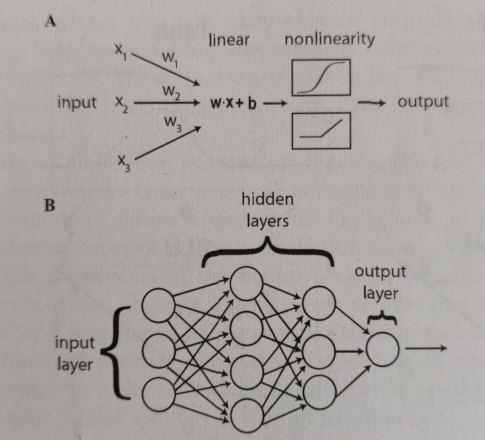
\includegraphics[width=0.7\linewidth]{gfx/Neuron}
	\caption{\itshape A) Neurons consist of a linear transformation that weights the importance of various inputs, followed by a non-linear activation function. B) Network architecture.}
	\label{fig:neuron}
\end{figure}




The linear transformation in almost all NNs takes the form of a dot product with a set of neuron-specific weights $\mw^{(i)} = (w^{(i)}_1,w^{(i)}_2,\dots,w^{(i)}_d)$ followed by re-centring with a neuron-specific bias $b^{(i)}$:
\be 
z^{(i)} = \mw^{(i)} \cdot \mx ü+ b^{(i)} = \textbf{x}^T \cdot \textbf{w}^{(i)},
\ee 
where $\textbf{x}=(1,\mx)$ and $\textbf{w}^{(i)} = (b^{(i)}, \mw^{(i)} )$.
\begin{mybox}{Choosing the right non-linearity}
 In terms of $z^{(i)}$ and the non-linear function $\sigma_i(z)$, we can write the full input-output function as 
\be 
\label{eq:dnnInputOutputfct}
a_i(\mx) = \sigma_i ( z^{(i)}).
\ee 
Historical choices of nonlinearities include step-functions (perceptrons), sigmoids (i.e. Fermi functions), and the hyperbolic tangent, cf. \ref{subsubsec:thresholdfct}. More recently, it has become more common to use rectified linear units (ReLUs), leaky rectified linear units (leaky ReLUs), and exponential linear units (ELUs). Different choice of non-linearities lead to different computational and training properties for neurons. The underlying reason for this is that we train neural nets using gd based methods, cf. \ref{sec:gd}, that require us to take derivatives of the neural input-output function with respect to the weights $\mw^{(i)}$ and the bias $b^{(i)}$.
\end{mybox}
Notice that the derivatives of the aforementioned non-linearities $\sigma(z)$ have very different properties. The derivative of the perceptron is zero everywhere except where the input is zero. This discontinuous behaviour makes it impossible to train perceptrons using gradient descent. For this reason, until recently the most popular choice of non-linearity was the $\tanh$ function or a sigmoid/Fermi function. However, this choice of non-linearity has a major drawback. When the input weights become large, as they often do in traingin, the activation functions saturates and the derivative of the output w.r.t. the weights tends to zero since $\partial \sigma /\partial z \rightarrow 0$ for $z\gg 1$. Such \emph{vanishing gradients} are a feature of any saturating function, making it harder to train deep networks. In contrast, for a non-saturating function such as ReLUs or ELUs, the gradients stay finite even for large inputs.

\subsubsection{Layering neurons to build deep networks: network architecture}
\label{subsubsec:dnnNetworkArchitecture}
The basic idea of all NNs is to layer neurons in a hierarchical fashion, the general structure of which is known as the \emph{network architecture}, compare \ref{fig:neuron}. In the simplest feed-forward networks, each neuron in the \emph{input layer} of the neurons takes the inputs $\textbf{x}$ and produces an output $a_i(\textbf{x})$ that depends on its current weights, see \ref{eq:dnnInputOutputfct}. The outputs of the input layer are then treated as the inputs to the next \emph{hidden layer}. This is usually repeated several times until one reaches the top or \emph{output layer}.
\begin{mybox}{Output layer and general architecture}
	The output layer is almost always a simple classifier of the form discussed before: a logistic regression \ref{sec:logisticRegression} or soft-max function \ref{subsec:logregSoftMax} in the case of categorical data (i.e. discrete labels) or a linear regression \ref{sec:linearRegression} layer in the case of continuous outputs. Thus, the whole neural network can be though of as a complicated nonlinear transformation of the inputs $\tx$ into an output $\hat{y}$ that depends on the weights and biases of all the neurons in the input, hidden, and output layers.
\end{mybox}
The use of hidden layers greatly expands the representation power (\emph{expressivity}) of a NN when compared with a simple soft-max or linear regression network, this is exemplified by the following theorem.
\begin{mybox}{Universal approximation theorem}
	A NN with a single hidden layer can approximate any continuous multi-input/multi-output function with arbitrary accuracy.
\end{mybox}
What does this mean and where does this come from ?\\
Note that by increasing the number of hidden neurons we can improve the approximation. Suppose we're given a function $f(x)$ which we'd like to compute to within some desired accuracy $ϵ>0$. The guarantee is that by using enough hidden neurons we can always find a neural network whose output $g(x)$ satisfies 
 \bse 
 \abs{g(x)-f(x)} < \epsilon,
 \ese 
  for all inputs $x$.
The approximation of the function works in the following way like a Riemann sum. Basically every pair of neurons in the hidden layer can be combined, via a combination of both weights, into a step function (or a sigmoid function which becomes a step function for large inputs). To be more precise, you can make every activation function into a step function by a clever combination of weights and bias if the activation function satisfies the following properties:\\
We do need to assume that $s(z)$ is well-defined as$z\rightarrow \infty$ and $z\rightarrow -\infty$. These two limits are the two values taken on by our step function. We also need to assume that these limits are different from one another. If they weren't, there'd be no step, simply a flat graph! But provided the activation function $s(z)$ satisfies these properties, neurons based on such an activation function are universal for computation (i.e. they are able to approximate any function).
\\
 Having $N$ pairs of hidden layer neuron pairs therefore gives you $N$ step function, which you can arrange beside each other, or overlapping. This is basically the approximation of the function. You Arrange step functions in such a way that they give you the function in a small section of the intervall. Therefore, basically neuron pairs in the hidden layer provide support functions as in analysis, which are step function approximating the true function for a small part of the interval. Therefore, by simply increasing the number of hidden layer neurons, you increase the number of step functions and decrease their width, resulting in a finer approximation of the function.\\
This makes use of the weighted combination $\sum_j w_j a_j$ output from the hidden neurons, however the function is given by the output layer, i.e. by the output $\sigma(\sum_j w_j a_j +b)$ where $b$ is the bias on the output neuron. How do you make the transition ?\\
The solution is to design a neural network whose hidden layer has a weighted output given by $\sigma^{-1}\circ f(x)$, such that the overall output will be a very good approximation of $\sigma\circ \sigma^{-1} \circ f(x) = f(x)$.
\\
If you have more inputs for one neuron, i.e. a many-input function $f(x_1,x_2,\dots)$, you get more weights, because every input $x_i$ has a weight $w_i$ associated with it which determines how much this input variable should contribute in this particular neuron, where every neuron also has one specific bias associated with it.\\
For two input variables:\\
 You can again create step function but this time in three dimensions (i.e. $x_1,x_2,g(x_1,x_2)$), which are called tower functions. These are constructed by introducing a second hidden layer. A pair of Neurons in the first hidden layer giving us a step-function in one direction can be combined with a pair of neurons giving us a step function in another direction (and so on) to create a tower function by a clever combination of heights of the two neuron pairs and bias of the neuron in the second hidden layer both of these pairs are connected to. Then, you can create any $3$ or $m$ dimensional function by stacking tower functions together. We can also make them as thin as we like, and whatever height we like. As a result, we can ensure that the weighted output from the second hidden layer approximates any desired function of two variables.
In particular, by making the weighted output from the second hidden layer a good approximation to $\sigma^{-1}\circ f$, we ensure the output from our network will be a good approximation to any desired function, $f$.\\
For $m$ input variables you need to have $m$ neuron pairs in the first hidden layer to feed into one respective neuron in the second hidden layer, where the former create all the step functions in the different dimensions by clever combination of parameters and the latter gives the output tower function in the given dimension.\\
For vector-valued functions, you simply compute the components of the vector separately via the above method and then put them into a vector.
\begin{mybox}{Conclusion}
We saw that we can approximate any function with just one hidden layer. Given this, you might wonder why we would ever be interested in deep networks, i.e., networks with many hidden layers. Can't we simply replace those networks with shallow, single hidden layer networks?\\
While in principle that's possible, there are good practical reasons to use deep networks. Deep networks have a hierarchical structure which makes them particularly well adapted to learn the hierarchies of knowledge that seem to be useful in solving real-world problems. Put more concretely, when attacking problems such as image recognition, it helps to use a system that understands not just individual pixels, but also increasingly more complex concepts: from edges to simple geometric shapes, all the way up through complex, multi-object scenes. Deep networks do a better job than shallow networks at learning such hierarchies of knowledge.
\end{mybox}
\subsubsection{Further on network architecture: How many layers is adequate for a problem ?}
\label{subsubsec:deepBestPracticeArchitecture}
Deep architectures are favourable for learning. Increasing the number of layers increases the number of parameters and hence the representational power of NNs. Indeed, recent numerical experiments suggest that as long as the number of parameters i larger than the number of data points, certain classes of NNs can fit arbitrarily labelled random noise samples. This suggests that large NNs of the kind used in practice can express highly complex function. Adding hidden layers is also though to allow neural nets to learn more complex features rom the data. Work on convolutional networks suggests that the first few layers of a neural network learn simple, ’low-level’ features thatare then combined into higher-level, more abstract features in the deeper layers.\\
\\
Choosing the exact network architecture for a NN remains an art that requires extensive numerical experimentation and intuition, and is often times problem-specific. Both the number of hidden layers and the number of neurons in each layer can affect the performance of a NN.
\begin{mybox}{Rule of thumb}
	A general rule of thumb that seems to be emerging is that the number of parameters in the NN should be large enough to prevent underfitting.
\end{mybox}
Empirically, the best architecture for a problem depends on the task, the amount and type of data that is available, and the computational resources at one's disposal. Certain architectures are easier to train, while others might be better at capturing complicated dependencies in the data and learning relevant input features. Finally, there architectures beyond simple deep, feed-forward NNs.
For example, modern NNs for image segmentation often incorporate ’skip connections’ that skip layers of NN. This allows information to directly propagate to a hidden or output layer, bypassing intermediate layers and often improving performance.

\subsubsection{Training deep networks}
\label{subsubsec:deepTraining}
\begin{mybox}{Training procedure}
	The training procedure is the same as we used for training simpler supervised learning algorithms such as logistic and linear regression, compare \ref{subsec:recipeML}:\\
	Construct a cost/loss function and then use gradient descent to minimize the cost function and find the optimal weights and biases. 
\end{mybox}
NNs differ from these simpler supervised procedures in that generally they contain multiple hidden layers that make taking the gradient computationally more difficult, this will be discussed in more detail via the \emph{backpropagation} algorithm for computing gradients in \ref{subsubsec:deepBackpropagation}.\\
\\
Like all supervised learning procedures, the first thing one must do to train a NN is to specify a loss function. Given a data point $(\tx_i,y_i)$, $\tx_i \in \mR^{d+1}$, the NN makes a prediction $\hat{y}_i(\tw)$, where $\tw$ are the parameters of the NN. Recall that in most cases, the top output layer of our NN is either a continuous predictor or a classifier that makes discrete (categorical) predictions. Depending on whether one wants to make continuous or categorical predictions, one must utilize a different kind of loss function.
\begin{enumerate} 
\item For continuous data, the loss functions that are commonly used to train NNs are identical to those used in linear regression:
\begin{enumerate}
	\item One is the mean squared error
	\be 
	\label{eq:deepCostSquaredError}
	E(\tw) = \frac{1}{n}\sum_{i=1}^n (y_i-\hat{y}_i(\tw) )^2, 
	\ee 
	where $n$ is the number of data points,
	\item and the mean-absolute error (i.e. $L_1$ norm) 
	\be 
	\label{eq:deepCostAbsoluteError} 
	E(\tw) = \frac{1}{n} \sum_i \abs{y_i - \hat{y}_i(\tw)}.
		\ee 
\end{enumerate}
The full cost function often includes terms that implement regularization (e.g. $L_1$ or $L_2$ regularizers).
\item For categorical data, the most commonly used loss function is the cross-entropy (\ref{eq:logregCrossEntropy} and \ref{eq:logregSoftMaxcostFct}), since the output layer is often taken to be a logistic classifier for binary data with two types of labels, or a soft-max classifier if there are more than two types of labels. As usual, these loss functions are often supplemented by aditional terms that implement regularization.
\end{enumerate}
Having defined an architecture and a cost function, we must now train the model. Similar to other supervised learning methods, we make use of gradient-descend based methods \ref{sec:gd} to optimize the cost function. Recall that the basic idea of GD is to update the parameters $\tw$ to move in the direction of the gradient of the cost function $\nabla_{\tw} E(\tw)$.\footnote{Most modern NN packages, such as Keras, allow te user to specify which of the optimizers discussed in \ref{sec:gd} they would like to use in order to train the NN. Depending on the architecture, data, and computation resources, different optimizers may work better on the problem, though vanilla SGD \ref{subsubsec:gdSGD} is a good first choice.}

\subsubsection{The Backpropagation algorithm}
\label{subsubsec:deepBackpropagation}








\chapter{Ideas for problems to work on}
\section{Physics problems}
\subsection{Cosmology}
\begin{enumerate}
	\item Maybe write a classification logistic regressor, or deep CNN to classify where dark matter halos have their boundary. It is very difficult to define a boundary of such a spread out object with confidence, maybe find criteria via classification ML technique ?
\end{enumerate}
\subsection{QFT}